\chapter{Secondo principio e cicli}

\section{Enunciati di Kelvin e Clausius}
\begin{fact}[Secondo principio della termodinamica, formulazione di Kelvin]
\textbf{Non esiste un processo che traformi \ul{interamente} calore in lavoro.}
\end{fact}

\begin{fact}[Secondo principio della termodinamica, formulazione di Clausius]
\textbf{Non esiste un processo il cui \ul{unico risulato} sia trasferire calore da una sorgente pi\`u fredda ad una pi\`u calda.}
\end{fact}

\begin{proposition}
Le due formulazioni del secondo principio sono equivalenti.
\end{proposition}
\begin{proof}
Mostrimo che le loro negazioni sono equivalenti:
\setlength{\leftmargini}{0cm}
\begin{itemize}
\item[$\boxed{\neg K\implies \neg C}$] Consideriamo il diagramma
\begin{figure}[!htb]
    \centering
    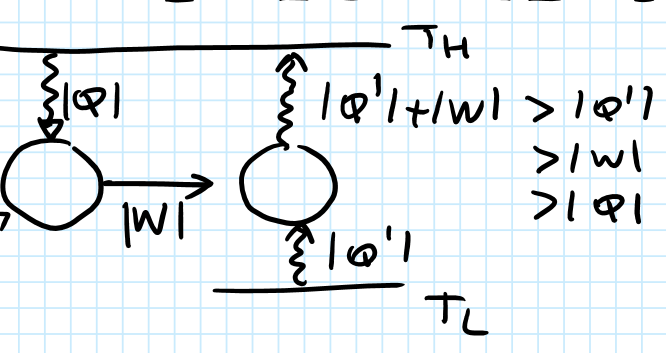
\includegraphics[width=5cm]{images/NonKelvin_Implica_NonClausius.png}
\end{figure}

Notiamo che $\abs{Q'}+\abs{W}>\max{\cpa{\abs{Q'},\abs{W}}}=\max{\cpa{\abs{Q'},\abs{Q}}}$. Considerando ora il sistema di due macchine come un insieme troviamo una macchina che trasferisce un calore $\abs{Q'}$ dala sorgente fredda alla sorgente calda, negando Clausius.
\item[$\boxed{\neg C\implies \neg K}$] Procediamo analogamente a prima
\begin{figure}[!htb]
    \centering
    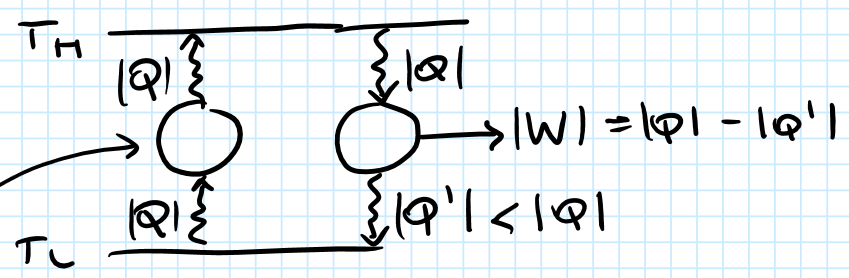
\includegraphics[width=7cm]{images/NonClausius_Implica_NonKelvin.png}
\end{figure}

e leggendo questo diagramma come un insieme la macchina avrebbe preso del calore $\abs Q-\abs{Q'}$ dalla sorgente $\theta_L$ e lo ha trasformato interamente in lavoro, negando Kelvin.
\end{itemize}
\setlength{\leftmargini}{0.5cm}
\end{proof}



\section{Cicli e temperatura assoluta}
\subsection{Processo ciclico}
\begin{definition}[Processo ciclico]
Un processo \`e \textbf{ciclico} se lo stato iniziale e finale sono lo stesso. Se qualcosa realizza un processo ciclico \`e detto \textbf{motore}.
\end{definition}

\begin{remark}[Diagramma di una macchina a due sorgenti]
Spesso torna comodo fare diagrammi come in figura
\begin{figure}[!htb]
    \centering
    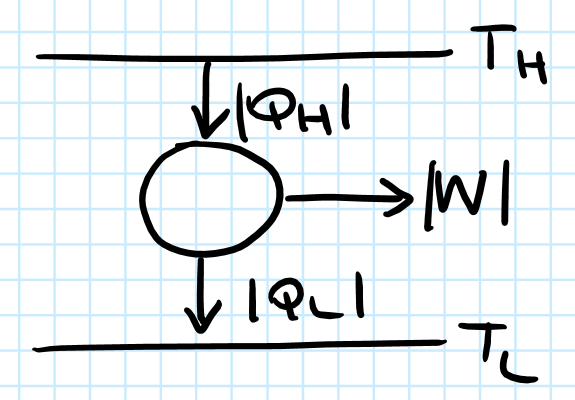
\includegraphics[width=4cm]{images/Diagramma_Ciclo.png}
\end{figure}

\end{remark}

\begin{remark}
Per un processo ciclico, $\Delta U=0$, dunque $Q=-W$.
\[-W=Q=Q_H+Q_L\]
dove $Q_H$ \`e il calore che il sistema acquista da una sorgente calda e $Q_L$ \`e il calore che acquista da una sorgente fredda\footnote{$Q_H$ \`e positivo e $Q_L$ \`e negativo.}. Notiamo che
\[\abs W=\abs{Q_H}-\abs{Q_L}.\]
\end{remark}

\begin{definition}[Efficienza]
L'\textbf{efficienza} di un processo ciclico \`e data da\footnote{Intuitivamente l'efficienza \`e una misura di quanto lavoro riesco a realizzare in proporzione a quanto calore abbiamo dovuto inserire nel sistema. L'altra forma ci dice che l'efficienza \`e una coversione perfetta eccetto per il calore che viene disperso senza diventare lavoro ($Q_L$).}
\[\eta=\frac{\abs W}{\abs{Q_H}}=1-\frac{\abs{Q_L}}{\abs{Q_H}}.\]
\end{definition}

\begin{definition}[Frigorifero e coefficiente di prestazione]
Un \textbf{frigorifero} \`e un motore che trasferisce calore da una sorgente fredda ad una calda. Il suo \textbf{coefficiente di prestazione} \`e dato da
\[COP=\frac{\abs{Q_L}}{\abs{W}}=\frac{1-\eta}\eta.\]
\end{definition}

\begin{definition}[Pompa di calore]
Una \textbf{pompa di calore} \`e una macchina volta a trasformare lavoro in calore verso la sorgente calda. La sua efficienza \`e quindi l'inversa di quella di un motore standard:
\[\frac{\abs{Q_H}}{\abs{W}}=\frac1\eta.\]
\end{definition}

\begin{theorem}[di Carnot]\label{TeoremaDiCarnot}
Un ciclo reversibile \`e il pi\`u efficiente che lavori tra due sorgenti $\theta_H$ e $\theta_L$.
\end{theorem}
\begin{proof}
Consideriamo due cicli $S$ ed $S'$ di cui $S$ reversibile. Per il primo principio $-W=\abs{Q_H}-\abs{Q_L}$ e $-W'=\abs{Q_H'}-\abs{Q_L'}$.\\
Con precisione arbitraria, siano $N$ ed $N'$ interi positivi tali che
\[\frac{\abs{Q_H}}{\abs{Q_H'}}\approx \frac{N'}{N}.\]
Facendo fare $N'$ cicli a $S'$ ed $N$ cicli reversibili \textit{al contrario}\footnote{qu\`i usiamo la reversibilit\`a. Se prima il sistema trasformava calore in lavoro con qualche perdita di calore ora il sistema riceve lavoro e un po' di calore per fornire calore alla sorgente calda} a $S$ troviamo
\[-W_{tot}=N'(-W')-N(-W)=N'(\abs{Q_H'}-\abs{Q_L'})-N(\abs{Q_H}-\abs{Q_L})\]
\[Q_{H,tot}=N'\abs{Q_H'}-N\abs{Q_H}\]
\[-Q_{L,tot}=N'\abs{Q_L'}-N\abs{Q_L}.\]
Per il primo principio, facendo lavorare in parallelo le due macchine
\[-W_{tot}=Q_{H,tot}+Q_{L,tot}.\]
Scegliendo $N$ ed $N'$ arbitrariamente grandi possiamo approssimare $Q_{H,tot}\approx 0$, e quindi
\[-W_{tot}\approx Q_{L,tot}.\]
Per la formulazione di Kelvin del secondo principio si ha che $-W_{tot}\leq0$\footnote{se cos\`i non fosse la macchina composta starebbe convertendo il calore $\abs{Q_{L,tot}}$ in lavoro sull'esterno $\abs{W_{tot}}$, contraddicendo il secondo principio.}, quindi $Q_{L,tot}\leq 0$, cio\`e
\[N'\abs{Q_L'}-N\abs{Q_L}\geq 0\coimplies \frac{N'}N\geq \frac{\abs{Q_L}}{\abs{Q_L'}}.\]
Passando al limite negli $N$ e $N'$ si ha che
\[\frac{\abs{Q_L}}{\abs{Q_H}}\leq \frac{\abs{Q_L'}}{\abs{Q_H'}}\implies \eta=1-\frac{\abs{Q_L}}{\abs{Q_H}}\geq 1-\frac{\abs{Q_L'}}{\abs{Q_H'}}=\eta'.\]
\end{proof}

\begin{corollary}[I cicli reversibili hanno la stessa efficienza]\label{CicliReversibiliHannoLaStessaEfficienza}
Tutti i cicli reversibili hanno la stessa efficienza.
\end{corollary}
\begin{proof}
Applicando il teorema abbiamo le due disuguaglianze scambiando i ruoli tra i due cicli.
\end{proof}


\subsection{Ciclo di Carnot}
Definiamo esplicitamente un ciclo reversibile:

\begin{definition}[Ciclo di Carnot]
Il \textbf{ciclo di Carnot} \`e composto dalle seguenti trasformazioni quasistatiche reversibili:
\begin{enumerate}
\item isoterma a temperatura $\theta_H$,
\item adiabatica da $\theta_H$ a $\theta_L$, 
\item isoterma a temperatura $\theta_L$,
\item adiabatica da $\theta_L$ a $\theta_H$.
\end{enumerate}
\end{definition}


\begin{remark}
Gli unici scambi di calore avvengono lungo l'isoterma, che ha senso solo a regime quasistatico (dato che il calore \`e uno scambio derivante da una differenza di energia).
\end{remark}

\begin{fact}
Il ciclo di Carnot \`e l'unico ciclo che effettua scambi in modo reversibile tra due sorgenti.
\end{fact}

\subsection{Temperatura assoluta}
Il teorema di Carnot (\ref{TeoremaDiCarnot}) ci suggerisce un modo per ridefinire la temperatura in termini della temperatura empirica senza bisogno di ricorrere ai gas:
\medskip

\noindent
Per il teorema di Carnot esiste $f$ tale che dopo un ciclo reversibile
\[\frac{\abs{Q_H}}{\abs{Q_L}}=f(\theta_L,\theta_H).\]
Collegando due tali processi facendo s\`i che il calore rilasciato dal primo sia quello assorbito dal secondo ricaviamo le equazioni
\[\frac{\abs{Q_3}}{\abs{Q_2}}=f(\theta_2,\theta_3),\quad\frac{\abs{Q_2}}{\abs{Q_1}}=f(\theta_1,\theta_2),\quad \frac{\abs{Q_3}}{\abs{Q_1}}=f(\theta_1,\theta_3),\]
dove $\theta_1\leq \theta_2\leq \theta_3$.\\
Segue dunque l'identit\`a
\[f(\theta_1,\theta_2)=\frac{f(\theta_1,\theta_3)}{f(\theta_2,\theta_3)}.\]
Derivando rispetto a $\theta_3$ ricaviamo
\begin{gather*}
0=\frac1{f(\theta_2,\theta_3)}\pp{\theta_3}{f}(\theta_1,\theta_3)-\frac{f(\theta_1,\theta_3)}{(f(\theta_2,\theta_3))^2}\pp{\theta_3}f(\theta_2,\theta_3)\\
\frac1{f(\theta_1,\theta_3)}\pp{\theta_3}{f}(\theta_1,\theta_3)=\frac1{f(\theta_2,\theta_3)}\pp{\theta_3}{f}(\theta_2,\theta_3).
\end{gather*}
Abbiamo dunque mostrato che $\frac1{f(\theta_1,\theta_3)}\pp{\theta_3}f(\theta_1,\theta_3)$ non dipende da $\theta_1$, cio\`e
\begin{gather*}
\pp{\theta_3}{}(\log(f(\theta_1,\theta_3)))=A(\theta_3)\\
\log(f(\theta_1,\theta_3))=B(\theta_3)+C(\theta_1),
\end{gather*}
dove $B(\theta_3)$ \`e una primitiva di $A(\theta_3)$.\\
Notiamo ora che $f(\theta,\theta)=1$ in quanto tanto calore viene rilasciato quanto viene assorbito se le sorgenti sono alla stessa temperatura.\\ 
Segue che $\log(f(\theta,\theta))=0$, cio\`e $B(\theta)=-C(\theta)$.
\[\log(f(\theta_1,\theta_3))=B(\theta_3)-B(\theta_1)\implies f(\theta_1,\theta_3)\pasgnlmath={g(\theta)=e^{B(\theta)}}\frac{g(\theta_3)}{g(\theta_1)}.\]
Possiamo dunque definire la \textbf{temperatura assoluta} come
\[T=g(\theta).\]
Tutto ci\`o che abbiamo detto fin'ora in termini della temperatura definita tramite gas continua ad essere valido per la temperatura assoluta.

\section{Entropia}
\subsection{Teorema di Clausius e definizione}
\begin{lemma}[Isoterme fibrano]\label{IsotermeFibrano}
Due isoterme non si incrociano
\end{lemma}
\begin{proof}
\`E un altro modo di esprimere lo 0-esimo principio.
\end{proof}

\begin{lemma}[Adiabatiche fibrano]\label{AdiabaticheFibrano}
Due curve adiabatiche non si incrociano.
\end{lemma}
\begin{proof}
Per assurdo supponiamo che due adiabatiche si incrocino. Trasformandole in un ciclo tramite una isoterma avremmo costruito una macchina che trasforma calore in lavoro senza effetti secondari, contraddicendo il secondo principio.

\begin{figure}[!htb]
    \centering
    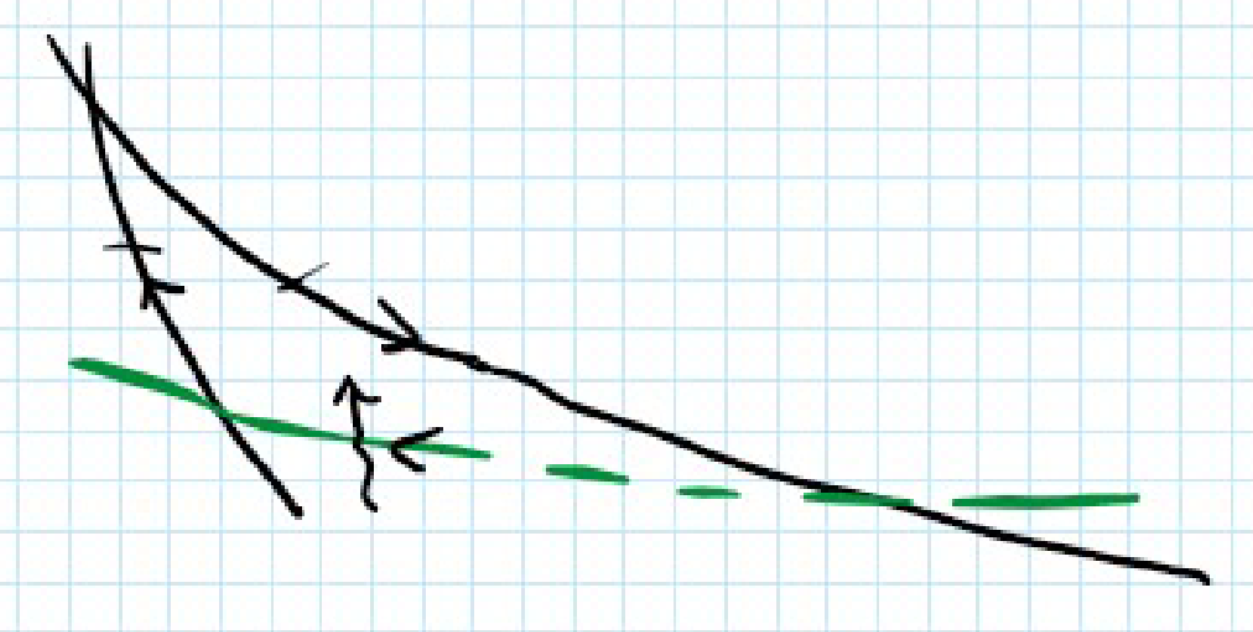
\includegraphics[width=5cm]{images/Adiabatiche_fibrano.png}
\end{figure}

\end{proof}


\begin{remark}[Clausius per cicli di Carnot]
In un ciclo di Carnot si ha che
\[\oint \frac{\delta Q}T=0.\]
\end{remark}
\begin{proof}
Dal teorema di Carnot (\ref{TeoremaDiCarnot}) e dalla definizione di temperatura empirica sappiamo che
\[\frac{\abs{Q_H}}{T_H}=\frac{\abs{Q_L}}{T_L},\]
cio\`e
\[0=\frac{Q_H}{T_H}+\frac{Q_L}{T_L}=\int_A^B\frac{\delta Q}T+\int_C^D\frac{\delta Q}T\pasgnl={$BC$ e $DA$ adiabatiche}\oint\frac{\delta Q}T.\]
\end{proof}

\begin{theorem}[Teorema di Clausius]\label{TeoremaClausius}
Per un qualsiasi ciclo reversibile si ha che
\[\oint\frac{\delta Q}T=0.\]
\end{theorem}
\begin{proof}
Approssimiamo il ciclo con tanti cicli di Carnot: per i lemma (\ref{IsotermeFibrano}) e (\ref{AdiabaticheFibrano}) evitiamo problemi di double counting, per costruire l'approssimazione basta scegliere due punti sul ciclo e sostituire il tratto del ciclo che li collega con la giunzione di una adiabatica, una isoterma e poi nuovamente una adiabatica, dove le adiabatiche sono determinate dagli stati in esame e l'isoterma \`e scelta in modo che il lavoro compiuto non cambi\footnote{poich\'e l'energia interna \`e una funzione di stato, garantire lo stesso lavoro automaticamente fornisce anche uguaglianze tra i calori}.

\begin{figure}[!htb]
    \centering
    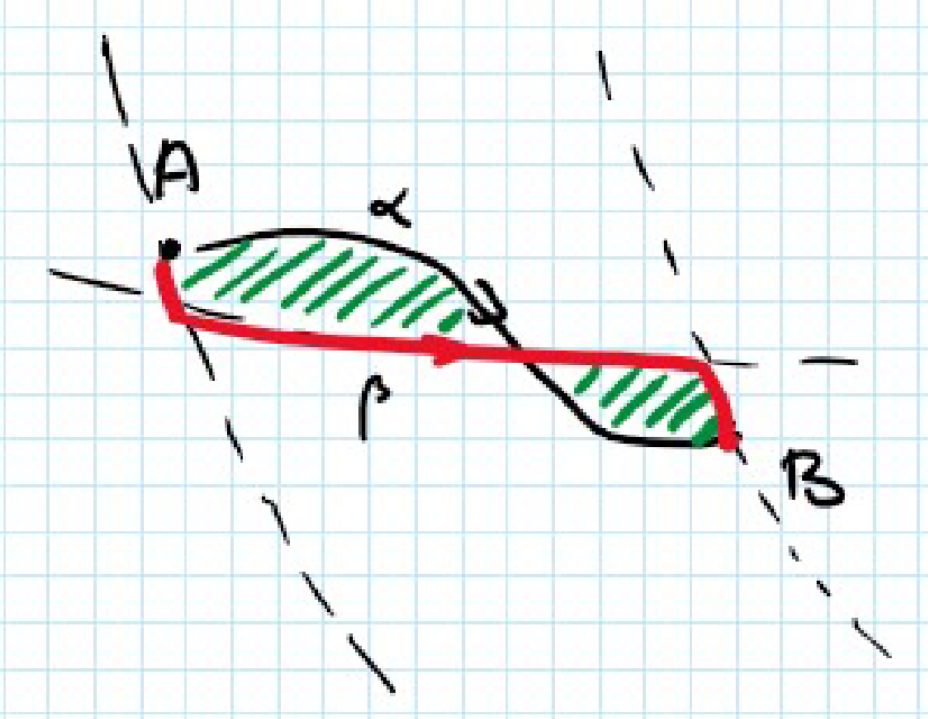
\includegraphics[width=4cm]{images/Come_Approssimare.png}
    \caption{Come viene sostituito un singolo tratto in modo da non cambiare il lavoro}
\end{figure}

\begin{figure}[!htb]
    \centering
    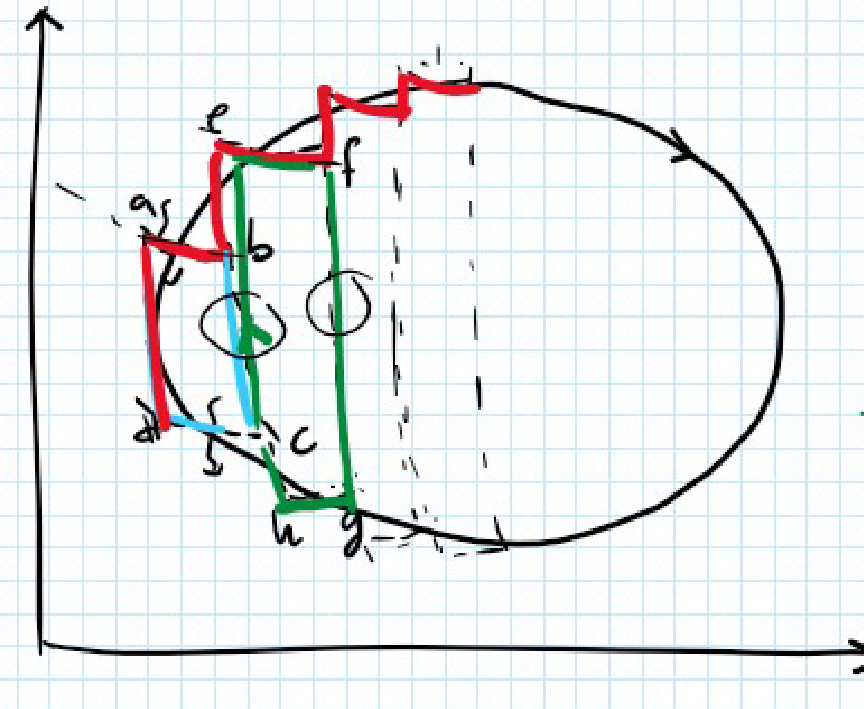
\includegraphics[width=5cm]{images/Dimostrazione_Teorema_Carnot.png}
    \caption{L'approssimazione del ciclo con tanti cicli di Carnot}
\end{figure}


\end{proof}

\begin{corollary}
La quantit\`a $\rbar{\int_A^B\frac{\delta Q}T}_{rev}$ \`e una funzione di stato.
\end{corollary}
\begin{proof}
Siano $\al$ e $\beta$ sono due \ul{processi reversibili} da $A$ a $B$. In quanto reversibili, \`e ben definito $\gamma=\ol \beta$ processo inverso di $\beta$. Per il teorema di Clausius (\ref{TeoremaClausius}) si ha che
\[0=\int_\al \frac{\delta Q}T+\int_\gamma\frac{\delta Q}T=\int_\al \frac{\delta Q}T-\int_\beta\frac{\delta Q}T,\]
come volevasi dimostrare.
\end{proof}

\noindent In luce di questo corollario \`e ben posta la seguente definizione:

\begin{definition}[Entropia]
Definiamo la \textbf{differenza di entropia} tra due stati $A$ e $B$ come\footnote{la notazione significa che per calcolare l'integrale scegliamo un qualsiasi processo reversibile che porta $A$ in $B$.}
\[\rbar{\int_A^B\frac{\delta Q}T}_{rev}=S_B-S_A.\]
In forma differenziale
\[dS=\frac{\delta Q}{T}_{rev}\]
\end{definition}

\begin{remark}
Se $\gamma$ \`e un processo che porta il sistema dallo stato $A$ allo stato $B$ in modo \textbf{non reversibile} allora \`e possibile che\[\int_A^B\frac{\delta Q}T\neq S_B-S_A.\]
La differenza di entropia tra i due stati \`e comunque ben definita, basta scegliere un secondo cammino reversibile da $A$ a $B$ e calcolare l'integrale lungo quel cammino.
\end{remark}

\begin{remark}
Se $A$ e $B$ sono stati sulla stessa adiabatica \[\underset{adiab.}{\int_A^B}\frac{\delta Q}T=0.\] 
Se l'adiabatica in questione \`e reversibile allora $S_A=S_B$.\\
Se l'adiabatica non \`e reversibile l'entropia potrebbe cambiare.
\end{remark}

\begin{remark}
Per un \underline{qualsiasi} ciclo (anche irreversibile), $\Delta S=0$, in quanto \`e una funzione di stato.
\end{remark}

\subsection{Entropia globale aumenta}
\begin{proposition}[Disuguaglianza di Clausius]\label{DisuguaglianzaClausius}
Sia $\Sigma$ un ciclo che acquista una quantit\`a di calore $\delta Q$ da una sorgente a temperatura $T_s$ e che produce una quantit\`a di lavoro $W$, allora \[\oint \frac{\delta Q}T\leq 0,\]
dove $T$ \`e la temperatura a cui lavora $\Sigma$.
\end{proposition}
\begin{proof}
Studiamo gli effetti secondari di $\Sigma$ \footnote{che necessariamente ci sono per il secondo principio.}.
Consideriamo il sistema composto da $\Sigma$ e una macchina di Carnot $\Sigma'$ definito come segue:\\
$\Sigma'$ assorbe un calore $\delta Q_s$ dalla sorgente $T_s$, produce del lavoro $W'$ e rilascia ad una temperatura $T$ il calore $\delta Q$ che riceve $\Sigma$.
\medskip

\noindent Calcolando la variazione di entropia per $\Sigma'$ ricaviamo che
\[0=\Delta S=\oint \frac{\delta Q_s}{T_s}+\oint -\frac{\delta Q}T\coimplies \frac1{T_s}\oint \delta Q_s=\oint \frac{\delta Q}T.\]
Consideriamo ora le due macchine insieme e calcoliamo l'energia:
\[Q_s=\oint \delta Q_s=-(W+W').\]
Per il secondo principio si ha che la quantit\`a sopra non \`e positiva\footnote{non possiamo convertire calore in lavoro senza altri effetti, ma possiamo convertire lavoro in calore senza problemi.}, dunque, sfruttando il fatto che $T_s>0$, si ha che
\[0\geq \frac1{T_s}\oint \delta Q_s=\oint \frac{\delta Q}T.\]
\end{proof}



\begin{theorem}[Variazione di entropia supera integrale sul percorso]\label{VariazioneEntropiaSuperaIntegrale}
Sia $\gamma$ un processo che porta lo stato $A$ nello stato $B$, potenzialmente in modo irreversibile, allora
\[\Delta S\geq \int_A^B\frac{\delta Q}T.\]
\end{theorem}
\begin{proof}
Sia $\al$ un processo reversibile che porta da $A$ a $B$ e sia $\beta$ il suo processo inverso.\\
Per la disuguaglianza di Clausius (\ref{DisuguaglianzaClausius}) si ha che
\[\under{=-\Delta S}{\int_\beta\frac{\delta Q}T}+\int_\gamma\frac{\delta Q}T\leq 0\implies \Delta S\geq \int_A^B\frac{\delta Q}T.\]
\end{proof}




\begin{proposition}[Secondo principio con entropia]
L'affermazione ``$\Delta S\geq 0$ per sistemi isolati" \`e equivalente al secondo principio della termodinamica.
\end{proposition}
\begin{proof}
Mostriamo le due implicazioni:
\setlength{\leftmargini}{0cm}
\begin{itemize}
\item[$\boxed{\impliedby}$] Assumendo il secondo principio abbiamo visto che vale il teorema (\ref{VariazioneEntropiaSuperaIntegrale}). Se un sistema \`e isolato, $\delta Q=0$, quindi 
\[\Delta S\geq \int \frac{\delta Q}T=0.\]
\item[$\boxed{\implies}$] Consideriamo per assurdo un processo che trasforma calore in lavoro senza altri effetti\footnote{Neghiamo la formulazione di Kelvin.}. 
La variazione di entropia del sistema sarebbe\footnote{il sistema perde calore per trasformarlo in lavoro, quindi il segno \`e negativo} 
\[\Delta S=\oint \frac{\delta Q}T=-\frac{\abs{Q}}T<0,\]
assurdo per ipotesi.
\end{itemize}
\setlength{\leftmargini}{0.5cm}


\end{proof}

\subsubsection{Differenziale dell'entropia}
\begin{remark}[Differenziale dell'entropia]
Poich\'e $U$ \`e una funzione di stato
\[dU=\delta Q+\delta W=\delta Q_{rev}+\delta W_{rev},\]
dunque
\[\boxed{dS=\rbar{\frac{\delta Q}T}_{rev}=\frac{\delta Q}T+\frac{\delta W-\delta W_{rev}}T}\]
Per il teorema (\ref{VariazioneEntropiaSuperaIntegrale}) si ha che $dS\geq \delta Q/T$, quindi per la forma sopra
\[\delta W\geq \delta W_{rev},\]
che \`e una riformulazione del teorema di Carnot (\ref{TeoremaDiCarnot}) se stiamo attenti ai segni.
\end{remark}

\begin{remark}
Scriviamo le forme $\delta Q=\sum_i A_idx_i$ e $\delta W=\sum_i X_idx_i$.\\
Sappiamo che questi non sono differenziali esatti, ma possiamo moltiplicare $\delta Q$ per $1/T$ e rendere quel differenziale esatto ($\delta Q/T=dS$). Questa \`e una manifestazione della proposizione (\ref{EsattezzaPfaff}).
\end{remark} 

\noindent
Ricalcando l'osservazione (\ref{IntegrabilitaPuntiRaggiungibili}) segue un'altra riformulazione del secondo principio:
\begin{proposition}[Secondo principio, formulazione di Caratheodory]\label{SecondoPrincipioCaratheodory}
Vicino ad ogni punto di equilibrio esistono infiniti punti non raggiungibili con adiabatiche reversibili.
\end{proposition}
\begin{proof}
NON DATA
\end{proof}

\begin{remark}
Se consideriamo una adiabatica reversibile $\delta Q=0$, gli stati vegono divisi in due regioni. In una regione troviamo punti raggiungibili tramite adiabatiche irreversibili, nell'altra troviamo punti irraggiungibili da qualsiasi adiabatica.
\end{remark}


\subsection{Sistema, Ambiente ed Entropia}

\begin{remark}
Un processo \`e reversibile se e solo se $\Delta S_{globale}=0$.
\end{remark}

\noindent
L'entropia pu\`o variare per due motivi: 
\begin{enumerate}
\item scambio di calore tra temperature diverse (causa \textit{esterna})
\item sono presenti attriti (causa \textit{interna})
\end{enumerate}

\begin{example}[Sistema e sorgente]
Consideriamo un universo formato unicamente da una sorgente a temperatura $T_s$ e un sistema che assorbe un un calore $Q$.
\begin{enumerate}
\item Supponiamo che il sistema non contenga attriti, cio\`e $\Delta S_{sist}^{(int)}$.\\ 
Per definizione di sorgente $\Delta S_{sorg}=-Q/T_s$, mentre
\[\Delta S_{sist}^{(ext)}\geq \int \frac{\delta Q}T\pasgnlmath\geq{T_s\geq T} \frac Q{T_s}.\]
\item Supponiamo che il sistema compia solo scambi di calore reversibili (cio\`e $\Delta S_{sorg}+\Delta S_{sist}^{(ext)}=0$), allora
\[\Delta S_{sorg}=\frac Q{T_s},\quad \Delta S_{sist}^{(ext)}=-\frac Q{T_s},\quad \Delta S_{sist}^{(int)}\geq 0.\]
\end{enumerate}
\end{example}


\begin{remark}[Cicli irreversibili]
Se un sistema fa un ciclo in modo irreversibile allora l'ambiente NON PU\`O aver fatto un ciclo in quanto altrimenti l'entropia non sarebbe aumentata.
\end{remark}

\section{Terzo principio}
\begin{fact}[Terzo principio della termodinamica]
\textbf{In un processo reversibile isotermo $\lim_{T\to 0}\Delta S=0$.}
\end{fact}
\begin{remark}
Stiamo dicendo che le isoterme per $T$ vicino a $0$ si avvicinano ad essere adiabatiche.
\end{remark}

\begin{remark}
Moralmente il principio dice che \`e difficile raffreddare verso temperature vicine allo 0 assoluto.
\end{remark}

\begin{remark}
Possiamo riformulare il principio affermando che ogni sistema ha la stessa entropia allo zero assoluto.
\end{remark}